

\begin{figure}[t!]
	\centering
	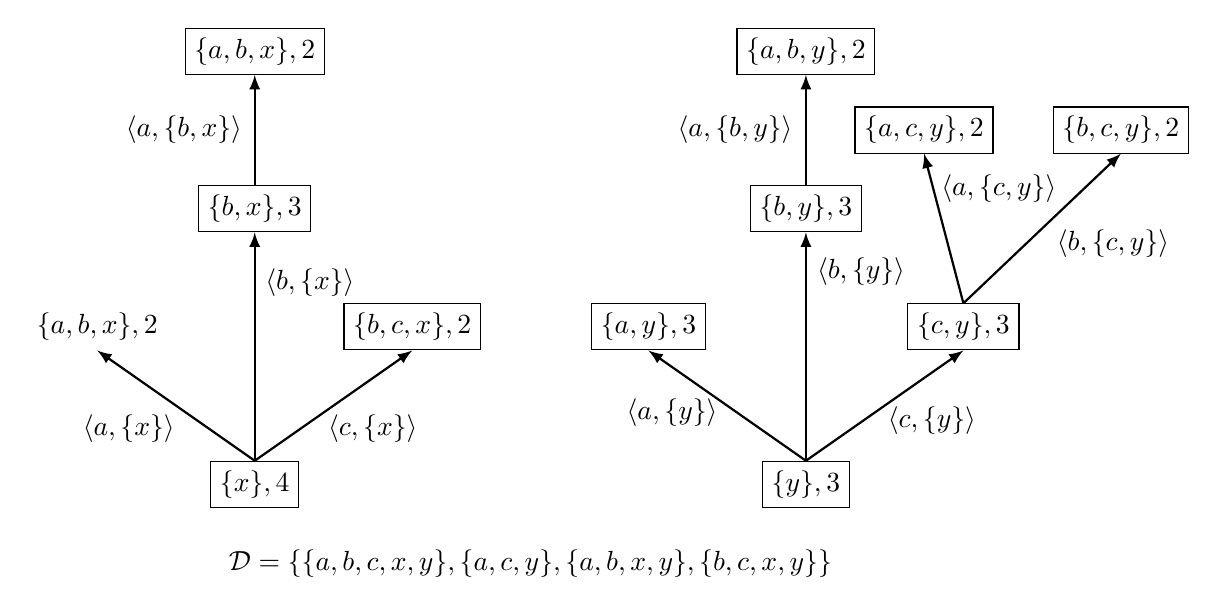
\begin{tikzpicture}[>=latex]%[>=triangle 45]
		\node(table) at (0,-1) {${\cal D}=\{\{a,b,c,x,y\}, \{a,c,y\}, \{a,b,x,y\}, \{b,c,x,y\}\}$};

		\node (x) [draw] at (-3.5,0) {$\{x\},4$};
		\node (y) [draw] at (3.5,0) {$\{y\},3$};
		\node (ax)  at (-5.5,2) {$\{a,b,x\},2$};
		\node (bx)  [draw] at (-3.5,3.5) {$\{b,x\},3$};
		\node (abx)  [draw] at (-3.5,5.5) {$\{a,b,x\},2$};
		\node (cx)  [draw] at (-1.5,2) {$\{b,c,x\},2$};
		\node (ay)  [draw] at (1.5,2) {$\{a,y\},3$};
		\node (by)  [draw] at (3.5,3.5) {$\{b,y\},3$};
		\node (aby)  [draw] at (3.5,5.5) {$\{a,b,y\},2$};
		\node (cy)  [draw] at (5.5,2) {$\{c,y\},3$};
		\node (acy)  [draw] at (5,4.5) {$\{a,c,y\},2$};
		\node (bcy)  [draw] at (7.5,4.5) {$\{b,c,y\},2$};
		\draw [->,thick] (x.north)--(ax.south) node[above, midway, xshift=-0.6cm, yshift=-0.6cm] {$\langle a, \{x\}\rangle$};
		\draw [->,thick] (x.north)--(bx.south) node[above, midway, xshift=0.7cm, yshift=0.5cm] {$\langle b, \{x\}\rangle$};
		\draw [->,thick] (x.north)--(cx.south) node[above, midway, xshift=0.5cm, yshift=-0.6cm] {$\langle c, \{x\}\rangle$};
		\draw [->,thick] (bx.north)--(abx.south) node[above, midway, xshift=-0.9cm, yshift=-0.3cm] {$\langle a, \{b,x\}\rangle$};
		\draw [->,thick] (y.north)--(ay.south) node[above, midway, xshift=-0.7cm, yshift=-0.4cm] {$\langle a, \{y\}\rangle$};
		\draw [->,thick] (y.north)--(by.south) node[above, xshift=0.7cm, yshift=-0.8cm] {$\langle b, \{y\}\rangle$};
		\draw [->,thick] (by.north)--(aby.south) node[above, midway, xshift=-0.9cm, yshift=-0.3cm] {$\langle a, \{b,y\}\rangle$};
		\draw [->,thick] (y.north)--(cy.south) node[above, midway, xshift=0.6cm, yshift=-0.5cm] {$\langle c, \{y\}\rangle$};
		\draw [->,thick] (cy.north)--(acy.south) node[above, midway, xshift=0.7cm, yshift=0.2cm] {$\langle a, \{c,y\}\rangle$};
		\draw [->,thick] (cy.north)--(bcy.south) node[above, midway, xshift=0.9cm, yshift=-0.5cm] {$\langle b, \{c,y\}\rangle$};
	\end{tikzpicture}

  \caption{\label{fig:capa:tree}
		\jlcm enumeration trees over an example dataset ${\cal D}$, with $\varepsilon=2$,
		in the \demoassoc case. Hence items in ${\cal B} = \{x,y\}$ are the only ones allowed as rules' consequent.
		An edge $\langle i, I \rangle$ represents an recursive invocation of \jlcm$(I, i)$.
		Only boxed nodes (closed itemsets satisfying the first-parent test) are returned.
		}
\end{figure}
